
\part[Instalação da playCB]
{Instalação da playCB}


\chapter[Instalação da playCB]
{Verificação de dependências da playCB}



\section{Resumo}


A playCB foi desenvolvida utilizando a linguagem C++, a API OpenGL e a biblioteca GLFW 2.7. A API OpenGL deve ser suportada pela placa de vídeo presente no computador, sendo exigido a versão 1.3 no mínimo. O tutorial para instalação tanto da GLFW quanto da própria playCB está disponível em detalhes no site Guia de Referência da playCB \footnote{\url{http://pt-br.playcb.wikia.com/wiki/Categoria:Instala\%C3\%A7\%C3\%A3o}}. Apesar da playCB ter sido desenvolvida em C++, o seu uso é focado primariamente para alunos que estejam a programar em C, ou seja, não é necessário conhecimento de C++ para utilizar a biblioteca, apenas utilizar a \emph{toolchain} do \emph{g++} para compilar.


%\begin{chapreferences}{1.}
%\bibliography{playcb}
%\bibliographystyle{plain}
%\nocite{cbook}
%\nocite{sb6}
%\nocite{glfw}
%\nocite{cppbook}

%\end{chapreferences}

\begin{chapreferences}{1}

\bibitem{sb6}
{\em OpenGL SuperBible}.
\newblock Pearson Education Inc, 6 edition, 2014.

\bibitem{glfw}
Marcus Geelnard and Camilla Berglund.
\newblock {\em GLFW - Reference guide}, 2010.
\newblock API version 2.7.

\bibitem{cbook}
Brian~W. Kernighan and Dennis~M. Ritchie.
\newblock {\em The C Programming Language}.
\newblock 1989.

\bibitem{cppbook}
Stanley~B. Lippman, Josés Lajoile, and Barbara Moo.
\newblock {\em C++ Primer}.
\newblock 2013.
\end{chapreferences}


\section{Plano Cartesiano}
\begin{figure}[ht]
  \centerline{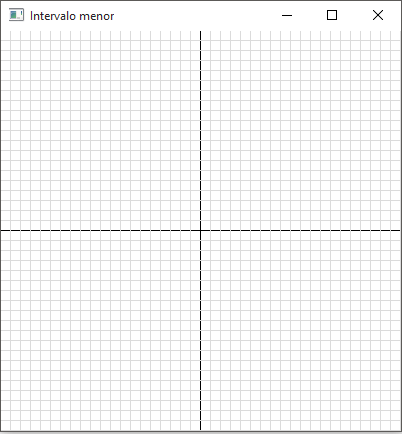
\includegraphics[width=.5\textwidth]{img/cap1_ex1.png}}
  \caption{Plano Cartesiano de -100 à 100}
  \label{fig:cap01_ex1}
\end{figure}
Esta prática se refere a exibir um Plano Cartesiano na tela com espaçamento de 5 em 5 unidades, tanto no eixo x quanto no eixo y. Com ela, o aluno poderá notar a importância da ordem de chamada de funções da playCB e a necessidade das funções \emph{AbreJanela} e \emph{Desenha}, além de verificar, com um exemplo simples, se a playCB foi corretamente bem instalada.
\lstinputlisting[caption=Código fonte de Plano Cartesiano, style=customc, label=lst:cap01_ex1]{src/ex1_PrimeiraJanela.cpp}
